\documentclass{standalone}
\usepackage{tikz}
\usetikzlibrary{patterns, positioning}


\begin{document}
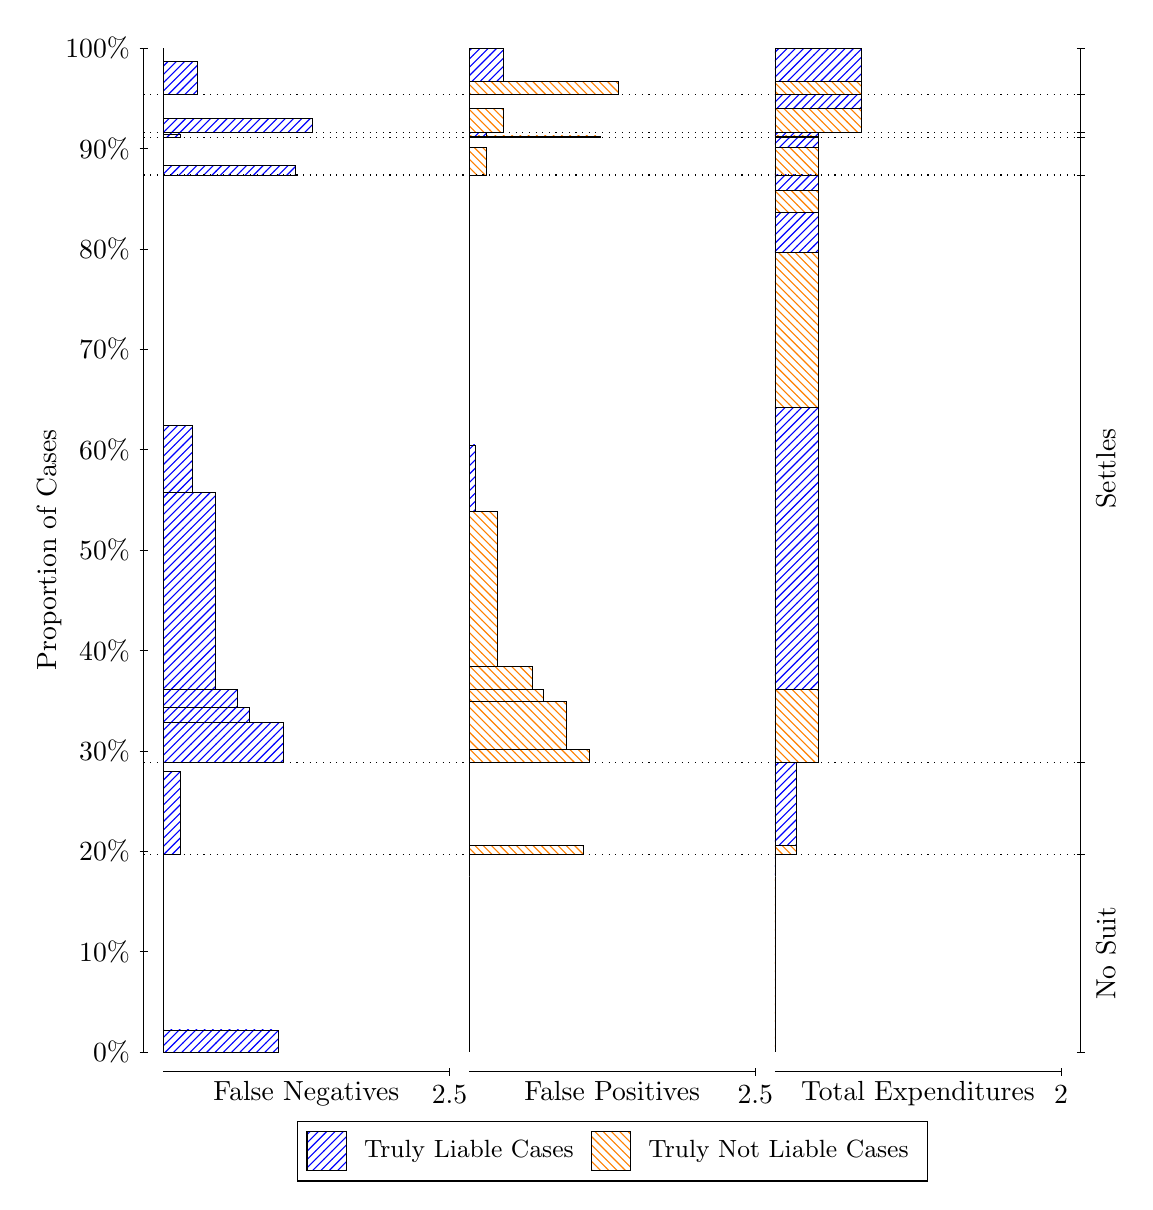
\begin{tikzpicture}
\draw[black, very thin] (1.5,1.75) -- (1.5,14.5);
\node[rotate=90, text=black, anchor=center] at (0.3, 8.125) {Proportion of Cases};
\draw[black, very thin] (1.45,1.75) -- (1.55,1.75);
\node[text=black, anchor=east] at (1.45, 1.75) {0\%};
\draw[black, very thin] (1.45,3.025) -- (1.55,3.025);
\node[text=black, anchor=east] at (1.45, 3.025) {10\%};
\draw[black, very thin] (1.45,4.3) -- (1.55,4.3);
\node[text=black, anchor=east] at (1.45, 4.3) {20\%};
\draw[black, very thin] (1.45,5.575) -- (1.55,5.575);
\node[text=black, anchor=east] at (1.45, 5.575) {30\%};
\draw[black, very thin] (1.45,6.85) -- (1.55,6.85);
\node[text=black, anchor=east] at (1.45, 6.85) {40\%};
\draw[black, very thin] (1.45,8.125) -- (1.55,8.125);
\node[text=black, anchor=east] at (1.45, 8.125) {50\%};
\draw[black, very thin] (1.45,9.4) -- (1.55,9.4);
\node[text=black, anchor=east] at (1.45, 9.4) {60\%};
\draw[black, very thin] (1.45,10.675) -- (1.55,10.675);
\node[text=black, anchor=east] at (1.45, 10.675) {70\%};
\draw[black, very thin] (1.45,11.95) -- (1.55,11.95);
\node[text=black, anchor=east] at (1.45, 11.95) {80\%};
\draw[black, very thin] (1.45,13.225) -- (1.55,13.225);
\node[text=black, anchor=east] at (1.45, 13.225) {90\%};
\draw[black, very thin] (1.45,14.5) -- (1.55,14.5);
\node[text=black, anchor=east] at (1.45, 14.5) {100\%};

\draw[black, very thin] (13.4,1.75) -- (13.4,14.5);
\draw[black, very thin] (13.35,1.75) -- (13.45,1.75);
\node[anchor=west] at (13.35, 1.75) {};
\draw[black, very thin] (13.35,4.2566) -- (13.45,4.2566);
\node[anchor=west] at (13.35, 4.2566) {};
\draw[black, very thin] (13.35,5.4295) -- (13.45,5.4295);
\node[anchor=west] at (13.35, 5.4295) {};
\draw[black, very thin] (13.35,12.888) -- (13.45,12.888);
\node[anchor=west] at (13.35, 12.888) {};
\draw[black, very thin] (13.35,13.363) -- (13.45,13.363);
\node[anchor=west] at (13.35, 13.363) {};
\draw[black, very thin] (13.35,13.432) -- (13.45,13.432);
\node[anchor=west] at (13.35, 13.432) {};
\draw[black, very thin] (13.35,13.908) -- (13.45,13.908);
\node[anchor=west] at (13.35, 13.908) {};
\draw[black, very thin] (13.35,14.5) -- (13.45,14.5);
\node[anchor=west] at (13.35, 14.5) {};

\draw[black, very thin, pattern color=blue, pattern=north east lines] (1.75,1.75) rectangle (3.2033,2.0306);
\draw[black, very thin, pattern color=orange, pattern=north west lines] (1.75,2.0306) rectangle (1.75,4.2566);
\draw[black, very thin, pattern color=blue, pattern=north east lines] (1.75,4.2566) rectangle (1.968,5.3104);
\draw[black, very thin, pattern color=orange, pattern=north west lines] (1.75,5.3104) rectangle (1.75,5.4295);
\draw[black, very thin, pattern color=blue, pattern=north east lines] (1.75,5.4295) rectangle (3.276,5.9328);
\draw[black, very thin, pattern color=blue, pattern=north east lines] (1.75,5.9328) rectangle (2.84,6.1258);
\draw[black, very thin, pattern color=blue, pattern=north east lines] (1.75,6.1258) rectangle (2.6947,6.3511);
\draw[black, very thin, pattern color=blue, pattern=north east lines] (1.75,6.3511) rectangle (2.404,8.8585);
\draw[black, very thin, pattern color=blue, pattern=north east lines] (1.75,8.8585) rectangle (2.1133,9.7066);
\draw[black, very thin, pattern color=orange, pattern=north west lines] (1.75,9.7066) rectangle (1.75,12.888);
\draw[black, very thin, pattern color=blue, pattern=north east lines] (1.75,12.888) rectangle (3.4213,13.011);
\draw[black, very thin, pattern color=orange, pattern=north west lines] (1.75,13.011) rectangle (1.75,13.363);
\draw[black, very thin, pattern color=blue, pattern=north east lines] (1.75,13.363) rectangle (1.968,13.411);
\draw[black, very thin, pattern color=orange, pattern=north west lines] (1.75,13.411) rectangle (1.75,13.432);
\draw[black, very thin, pattern color=blue, pattern=north east lines] (1.75,13.432) rectangle (3.6393,13.605);
\draw[black, very thin, pattern color=orange, pattern=north west lines] (1.75,13.605) rectangle (1.75,13.908);
\draw[black, very thin, pattern color=blue, pattern=north east lines] (1.75,13.908) rectangle (2.186,14.327);
\draw[black, very thin, pattern color=orange, pattern=north west lines] (1.75,14.327) rectangle (1.75,14.5);
\draw[black, very thin, pattern color=orange, pattern=north west lines] (5.6333,1.75) rectangle (5.6333,3.976);
\draw[black, very thin, pattern color=blue, pattern=north east lines] (5.6333,3.976) rectangle (5.6333,4.2566);
\draw[black, very thin, pattern color=orange, pattern=north west lines] (5.6333,4.2566) rectangle (7.0867,4.3756);
\draw[black, very thin, pattern color=blue, pattern=north east lines] (5.6333,4.3756) rectangle (5.6333,5.4295);
\draw[black, very thin, pattern color=orange, pattern=north west lines] (5.6333,5.4295) rectangle (7.1593,5.5904);
\draw[black, very thin, pattern color=orange, pattern=north west lines] (5.6333,5.5904) rectangle (6.8687,6.2039);
\draw[black, very thin, pattern color=orange, pattern=north west lines] (5.6333,6.2039) rectangle (6.578,6.3585);
\draw[black, very thin, pattern color=orange, pattern=north west lines] (5.6333,6.3585) rectangle (6.4327,6.6453);
\draw[black, very thin, pattern color=orange, pattern=north west lines] (5.6333,6.6453) rectangle (5.9967,8.6108);
\draw[black, very thin, pattern color=blue, pattern=north east lines] (5.6333,8.6108) rectangle (5.706,9.4589);
\draw[black, very thin, pattern color=blue, pattern=north east lines] (5.6333,9.4589) rectangle (5.6333,12.888);
\draw[black, very thin, pattern color=orange, pattern=north west lines] (5.6333,12.888) rectangle (5.8513,13.239);
\draw[black, very thin, pattern color=blue, pattern=north east lines] (5.6333,13.239) rectangle (5.6333,13.363);
\draw[black, very thin, pattern color=orange, pattern=north west lines] (5.6333,13.363) rectangle (7.3047,13.384);
\draw[black, very thin, pattern color=blue, pattern=north east lines] (5.6333,13.384) rectangle (5.8513,13.432);
\draw[black, very thin, pattern color=orange, pattern=north west lines] (5.6333,13.432) rectangle (6.0693,13.736);
\draw[black, very thin, pattern color=blue, pattern=north east lines] (5.6333,13.736) rectangle (5.6333,13.908);
\draw[black, very thin, pattern color=orange, pattern=north west lines] (5.6333,13.908) rectangle (7.5227,14.081);
\draw[black, very thin, pattern color=blue, pattern=north east lines] (5.6333,14.081) rectangle (6.0693,14.5);
\draw[black, very thin, pattern color=orange, pattern=north west lines] (9.5167,1.75) rectangle (9.5167,3.976);
\draw[black, very thin, pattern color=blue, pattern=north east lines] (9.5167,3.976) rectangle (9.5167,4.2566);
\draw[black, very thin, pattern color=orange, pattern=north west lines] (9.5167,4.2566) rectangle (9.7892,4.3756);
\draw[black, very thin, pattern color=blue, pattern=north east lines] (9.5167,4.3756) rectangle (9.7892,5.4295);
\draw[black, very thin, pattern color=orange, pattern=north west lines] (9.5167,5.4295) rectangle (10.062,6.3585);
\draw[black, very thin, pattern color=blue, pattern=north east lines] (9.5167,6.3585) rectangle (10.062,9.9393);
\draw[black, very thin, pattern color=orange, pattern=north west lines] (9.5167,9.9393) rectangle (10.062,11.905);
\draw[black, very thin, pattern color=blue, pattern=north east lines] (9.5167,11.905) rectangle (10.062,12.408);
\draw[black, very thin, pattern color=orange, pattern=north west lines] (9.5167,12.408) rectangle (10.062,12.695);
\draw[black, very thin, pattern color=blue, pattern=north east lines] (9.5167,12.695) rectangle (10.062,12.888);
\draw[black, very thin, pattern color=orange, pattern=north west lines] (9.5167,12.888) rectangle (10.062,13.239);
\draw[black, very thin, pattern color=blue, pattern=north east lines] (9.5167,13.239) rectangle (10.062,13.363);
\draw[black, very thin, pattern color=orange, pattern=north west lines] (9.5167,13.363) rectangle (10.062,13.384);
\draw[black, very thin, pattern color=blue, pattern=north east lines] (9.5167,13.384) rectangle (10.062,13.432);
\draw[black, very thin, pattern color=orange, pattern=north west lines] (9.5167,13.432) rectangle (10.607,13.736);
\draw[black, very thin, pattern color=blue, pattern=north east lines] (9.5167,13.736) rectangle (10.607,13.908);
\draw[black, very thin, pattern color=orange, pattern=north west lines] (9.5167,13.908) rectangle (10.607,14.081);
\draw[black, very thin, pattern color=blue, pattern=north east lines] (9.5167,14.081) rectangle (10.607,14.5);
\draw[black, dotted] (1.5,4.2566) -- (13.4,4.2566);
\draw[black, dotted] (1.5,5.4295) -- (13.4,5.4295);
\draw[black, dotted] (1.5,12.888) -- (13.4,12.888);
\draw[black, dotted] (1.5,13.363) -- (13.4,13.363);
\draw[black, dotted] (1.5,13.432) -- (13.4,13.432);
\draw[black, dotted] (1.5,13.908) -- (13.4,13.908);
\draw[black, very thin] (1.75,1.5) -- (5.3833,1.5);
\node[text=black, anchor=north] at (3.5667, 1.5) {False Negatives};
\draw[black, very thin] (5.3833,1.45) -- (5.3833,1.55);
\node[text=black, anchor=north] at (5.3833, 1.45) {2.5};

\draw[black, very thin] (5.6333,1.5) -- (9.2667,1.5);
\node[text=black, anchor=north] at (7.45, 1.5) {False Positives};
\draw[black, very thin] (9.2667,1.45) -- (9.2667,1.55);
\node[text=black, anchor=north] at (9.2667, 1.45) {2.5};

\draw[black, very thin] (9.5167,1.5) -- (13.15,1.5);
\node[text=black, anchor=north] at (11.333, 1.5) {Total Expenditures};
\draw[black, very thin] (13.15,1.45) -- (13.15,1.55);
\node[text=black, anchor=north] at (13.15, 1.45) {2};

\node[text=black, centered, rotate=90] at (13.72, 3.0033) {No Suit};

\node[text=black, centered, rotate=90] at (13.72, 9.1587) {Settles};





\draw (7.449999999999999,1.5) node[draw=none] (baseCoordinate) {};
\begin{scope}[align=center]
        \matrix[scale=0.5, draw=black, below=0.5cm of baseCoordinate, nodes={draw}, column sep=0.1cm]{
            \node[rectangle, draw, minimum width=0.5cm, minimum height=0.5cm, pattern color=blue, pattern=north east lines] {}; &
            \node[draw=none, font=\small, text=black] (B) {Truly Liable Cases}; &
            \node[rectangle, draw, minimum width=0.5cm, minimum height=0.5cm, pattern color=orange, pattern=north west lines] {}; &
            \node[draw=none, font=\small, text=black] (B) {Truly Not Liable Cases}; \\
            };
\end{scope}

\end{tikzpicture}
\end{document}